%%%%%%%%%%%%%%%%%%%%%%%%%%%%%%%%%%%%%%%%%%%%%%%%%%%%%%%%%
\section{Algoritmo propuesto}
\label{posing:method}
%%%%%%%%%%%%%%%%%%%%%%%%%%%%%%%%%%%%%%%%%%%%%%%%%%%%%%%%%

El objetivo es ser capaz de modificar toda la anatomía interna y externa de un modelo anatómico virtual usando una representación superficial. \new{En el mundo de los gráficos por computados, tradicionalmente, se utilizado la animación esqueletal para transformar la superficie de modelos articulados.}\todo{1. Indicar muy brevemente las ventajas de la animación esqueletal alineadas con los objetivos. 2. Indicar porque la técnica clasica no se puede utilizar. La extendemos para anatomía interna. }

\todo{1. No usamos las técnicas clásicas porque no tiene en cueta la anatomía interna. 2. No entiendo la seguna parte de la frase}
\del{En lugar de utilizar las técnicas clásicas de animación esqueletal, se ha propuesto una nueva manera novedosa de animar anatomías de personajes de manera eficiente, ya que para animar todos los tejidos de forma separada implicaría que habría que realizar las etapas de la animación para cada tejido de manera independiente y que no se podría asegurar que se generaran auto colisiones entre ellos.}

\new{La idea principal que hay detrás del algoritmo propuesto} es de calcular un campo de desplazamientos \new{continuo} \todo{si no es continuo todo lo que dices a continuación no sirve} en el interior del paciente virtual \new{y utilizarlo para transformar las estructuras internas}. Esto permite \del{poder mover}\new{deformar} los tejidos de \new{forma independiente y, aun así, garantizar que estos se muevan solidariamente, asegurando que no se produzcan colisiones.}\del{ solidaria sin necesidad de realizar cálculos independientes y asegurar de esta manera que no se producirá nuevas colisiones.} \todo{cuentalo luego}\del{Además, esta forma de trabajar permite no sólo animar representaciones superficiales, sino que es factible animar modelos volumétricos.}



\todo{1. todo automático menos la selección de la pose. 2. Indicar que la animación tradicional confía en el artista en muchos paso}
Otro de los objetivos propuestos para este algoritmo es que el método fuera totalmente automático sin necesidad de depender de las habilidades artísticas de un profesional. Para ello se ha buscado en la bibliografía aquellas técnicas automáticas que puedan ser útiles como se puede leer en el estado del arte \ref{art:anatomy} y se han adaptado para ser incorporadas en este método.

Como se ha especificado en la sección \ref{posing:req}, esta técnica ha sido diseñada para funcionar con anatomías incompletas siendo sólo obligatorio que la piel y los huesos estén correctamente identificados. \todo{1. Esta frase no se como se enlaza con la anterior. 2. repites la idea de etapas automaticas que ya habías explicado en el paso anterior.}El algoritmo propuesto sigue la línea del cauce clásico de animación esqueletal, modificando aquellas etapas con el objetivo de que sea automático y permita modelos incompletos.

\todo{Relata la idea principal. Crear el despalazamiento a partir del movimiento de los huesos. 2. Expliar la diferencia enter hueso virtual y tejido oseo. 3. Una vez acabado el parrafo lee toda esta into para que no haya cosas duplicadas. }

\del{Por tanto, el algoritmo propuestose puede dividir en las siguientes etapas}. \new{A continuación se detallan las etapas en las que se divide el algoritmo} (ver Fig. \ref{fig:Resumen}). \new{Tal y como puede comprobarse, muchas de las etapas, se inspiran en la animación esquela tal tradicional}:
\begin{itemize}
	\item \emph{Rigging}\todo{Déjalo en ingles, pero en el estado del arte, cuando se hable de rigging, mete un nota al pie donde digas lo que es }: \todo{Se que has traducido del ingles, pero tio!!! que tu hablas castellano} \del{Un esqueleto virtual predefinido \del{es} ajustado a la anatomía del personaje.}\new{En esta es etapa, se adapta un esqueleto virtual a la anatomia del paciente.} El algoritmo usa el tejido óseo para calcular el centro de rotación de cada articulación (sec. \ref{art:rigging}) del hueso virtual.
     \item \emph{Volumetrización}: \new{En esta etapa, se genera una malla de tetraedros que volumetriza el interior del modelo. Esta malla se genera a partir de la de la piel y los huesos del paciente virtual y} \del{Esta malla } servirá para definir un campo de desplazamientos continuo, que se asociará con el movimiento de los huesos.
\item \emph{Pesado}: A continuación, se calcula de manera automática la influencia de cada hueso del tejido oseo a cada vértice de la malla de tetraedros. 
\item \emph{Mapeado}: Todos los demás tejidos son asignados a los tetraedros de la malla volumétrica. 
\item \emph{Selección de pose}: En esta etapa, el movimiento de los huesos virtuales es transferido a la malla de tetraedros usando una técnica estándar de \emph{skinning}: \ac{LBS}, \ac{DQS} o \ac{COR}. 
\todo{Esto no es la primera vez que te lo digo. Cuando utilices la pasiva que suene natural!!!}
Después, el movimiento de estos tetraedros\new{, se transferirá} \del{será} aplicado a los tejidos del modelo \del{según estén relacionados}. Esta etapa puede ser interactiva dejando al usuario elegir la pose, o puede usarse otras técnicas de animación como pueden ser \ac{MoCap} o cinemática inversa entre otros con el objetivo de que la etapa se ejecute de manera automática.\todo{La cinemática inversa no es automática, es interactiva. }
\item \emph{Optimización}: \del{Adicionalmente,}\new{De forma opcional,} se permite al usuario refinar el resultado obtenido con la intención de preservar el volumen del modelo anatómico.\todo{La frase es rara. Creo que con la intención  no suena bien.}
\end{itemize}

\todo{rehacer imagen resumen}
\todo{hazla más grande}
\begin{figure*}[!th]
   \centering
    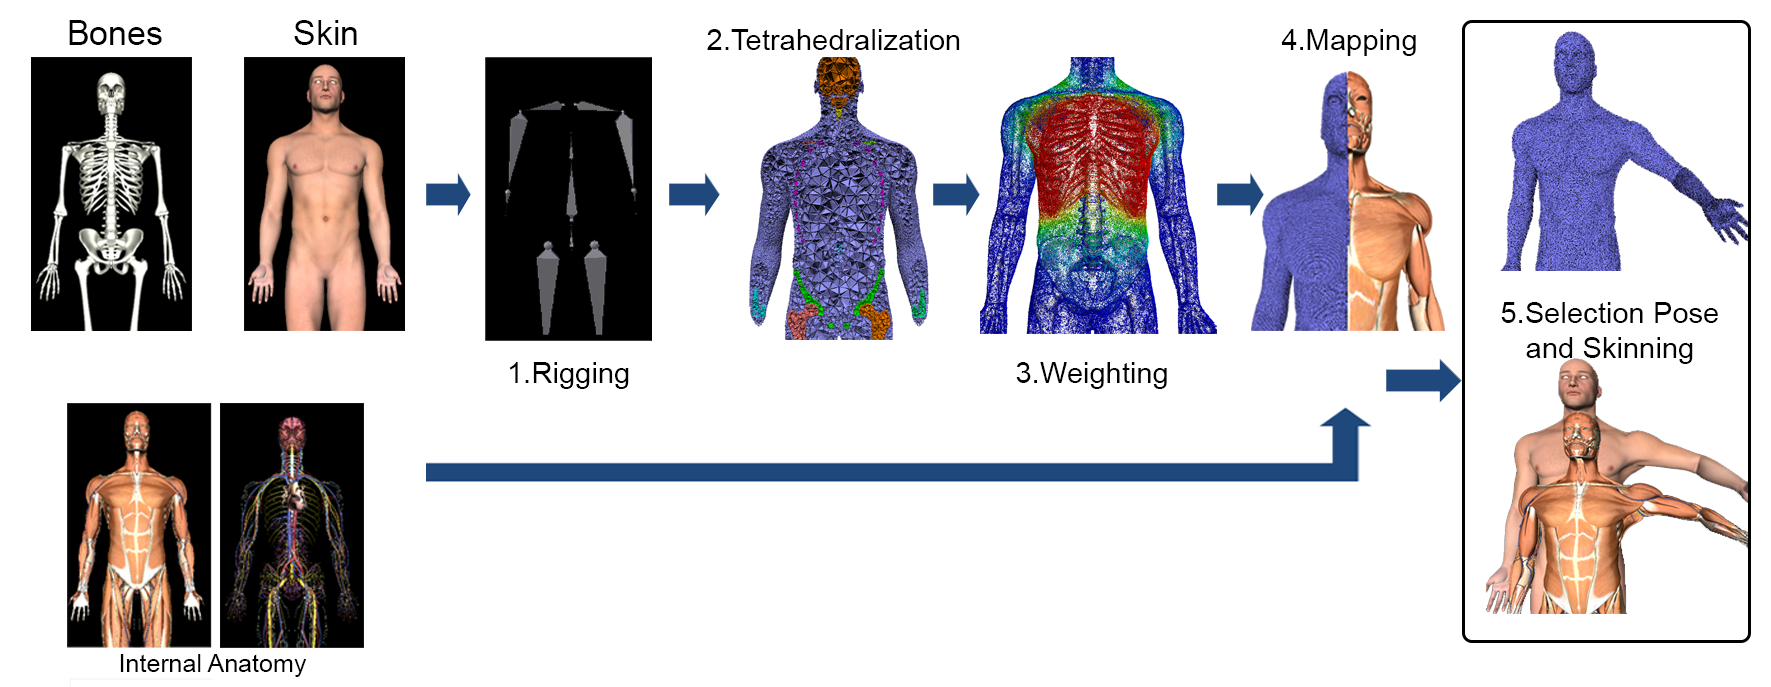
\includegraphics[width=0.9\textwidth]{IMG/resumencasa2.png}
    \caption{Perspectiva general del algoritmo propuesto}
		\label{fig:Resumen}
\end{figure*}


%

A continuación, se describirá detalladamente cada una de las etapas por separado, remarcando aquellas innovaciones y adaptaciones hechas específicamente para esta solución.



%%%%%%%%%%%%%%%%%%%%%%%%%%%%%%%%%%%%%%%%%%%%%%%%%%%%%%
\subsection{Rigging}
\label{posing:rigging}
%%%%%%%%%%%%%%%%%%%%%%%%%%%%%%%%%%%%%%%%%%%%%%%%%%%%%%
De manera similar a los huesos reales, un esqueleto virtual permite el movimiento del personaje que se quiere animar. El esqueleto virtual se representa como un conjunto jerarquizado de huesos virtuales conectados entre sí. El movimiento de cada hueso virtual está definido por una rotación teniendo en cuenta el centro de rotación de la articulación. Este movimiento puede ser fácilmente ampliable a otros tipos de movimientos más complejos discutidos en la sección \ref{art:rigging}.


En esta etapa, el método ajusta un esqueleto virtual predefinido al tejido oseo del modelo, y se define un centro de rotación para cada articulación teniendo en cuenta la forma del hueso real.
\todo{1. Explica que en la bibliografia existen técnicas que crean en el esqueleto y otras que ajustan uno existente. 2. En Rasimas los pacientes se generan registrando datos reales en el modelo del Zygote. 3. Redacta lo que viene a  continuación para que este bien ligado con esto. 4. Tienes que encuenta que etiquetas el modelo en reposo. Recuerda el documento que nos pasó antoine. De hecho puedes poner este docuemento en el apendice y citarlo. De verdad falta mucha información}
Para ello, se han identificado manualmente unas regiones significativas de cada hueso del que se quiere calcular el centro de rotación de la articulación en cuestión. En la figura \ref{fig:humero}, se pueden apreciar las distintas regiones seleccionadas para una muestra de diferentes huesos.
Estas zonas etiquetadas son identificadas en el modelo anatómico de entrada (normalmente procedente de imágenes médicas) y \del{se usan} \del{son usadas} para calcular el centro de rotación de las distintas articulaciones. Las zonas rojas que se muestran en la figura \ref{fig:humero} sirven para calcular el centroide que se usará como punto de rotación para cada hueso. Con este punto y los puntos obtenidos de la misma manera de las áreas de color azul y verde se puede estimar dos vectores ortogonales (el tercer eje se calcula mediante el producto vectorial de ambos) que servirán para definir el sistema local de referencia para ese hueso.
Se asume que el modelo que venga como entrada de las etapas anteriores se puedan identificar las mismas regiones y se presenten en la misma posición anatómica del paciente. Además, para hacer estos cálculos más robustos, el algoritmo considerará (cuando sea posible) regiones más grandes, minimizando los posibles defectos de un mal registro. Este proceso es específico para cada hueso virtual y puede ser fácilmente ampliable para todo tipo de huesos. La explicación de cada hueso que se ha utilizado en la presente tesis se podrá consultar en el anexo \ref{anexo:rigging}. 
\todo{Creo que tienes que mejorar como enlazas las ideas en este parrafo.}
Esta etapa concreta ha sido desarrollada por \emph{Antonie Serruier}, miembro del proyecto \ac{RASimAs}, en colaboración con el autor de esta tesis basada en anteriores trabajos \cite{QUIJANO20131703}.
\todo{revisar los colores de las fotos}
\todo{Aumenta el tamño de todas las imágnes}

\todo{indica el código de colores}
\begin{figure}
   \centering
    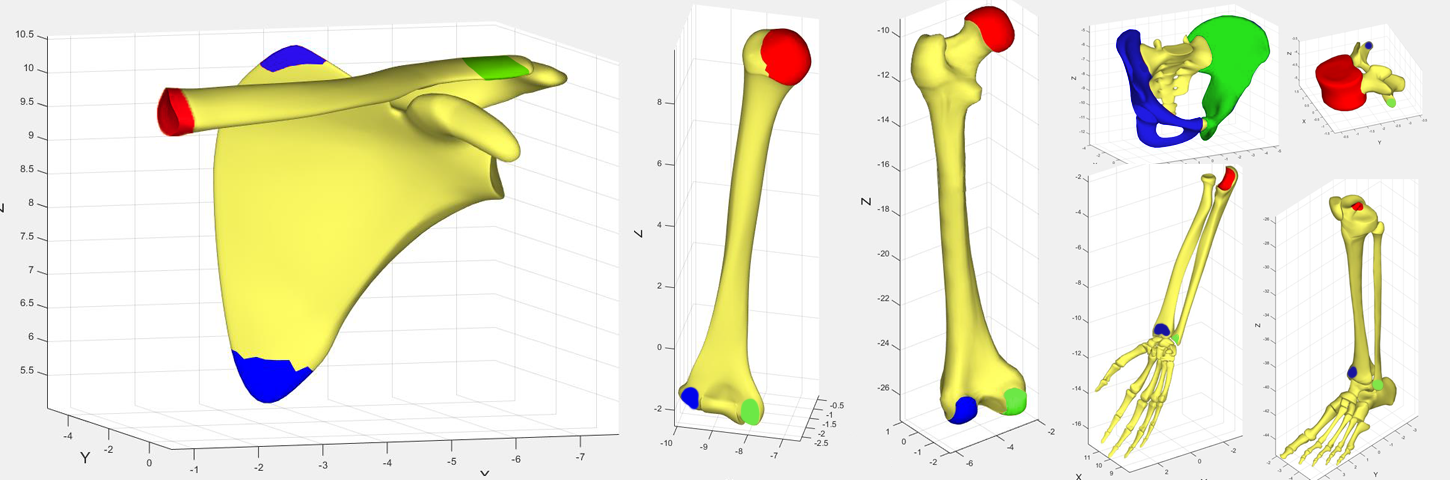
\includegraphics[width=0.8\textwidth]{IMG/rigshoulder.png}
    \caption{\del{Representaciones de algunos huesos}\new{La imagen muestra los huesos del modelo de referencia antes de registrar los datos del paciente}. Las áreas coloreadas \del{son utilizadas}\new{se utilizan}  para calcular el sistema de referencia de cada \del{\emph{joint}} articulación.}
\label{fig:humero}
\end{figure}


%%%%%%%%%%%%%%%%%%%%%%%%%%%%%%%%%%%%%%%%%%%%%%%%%%%%%%
\subsection{Volumetrización}
\label{posing:volumetrizacion}
%%%%%%%%%%%%%%%%%%%%%%%%%%%%%%%%%%%%%%%%%%%%%%%%%%%%%%
%
Como se ha introducido anteriormente, el objetivo es crear un campo de desplazamientos interno para poder mover toda la anatomía del personaje. El algoritmo discretiza el interior del modelo virtual utilizando \del{tejido de} la piel \new{y el tejido oseo} como referencia,\new{obteniendo} \del{Con ello es posible calcular una} malla volumétrica formada por tetraedros. Esta malla de tetraedros es una pieza clave del algoritmo \new{que se utilizará para calcular el citado campo de desplazamientos.}\del{ ya que será utilizada en} La siguiente etapa (sec. \ref{posing:Pesado}) \del{que servirá para}  calculará la influencia del movimiento de cada hueso en los vértices de los tetraedros, \new{de forma que el movimiento de los huesos afecte a los vértices del la malla volumétrica. El campo de desplazamientos se obtendrá de forma implícita interpolando el desplazamiento de los vértices en el interior de los tetraedros, mediante el uso de coordenadas baricéntricas.}  \del{Después, esta malla será donde se calcule el campo de desplazamiento (Sec. \ref{posing:Poses}). También, el campo de desplazamientos guiará la animación del modelo virtual gracias al cálculo del mapeado entre los tetraedros generados en esta etapa y los distintos tejidos (Sec. \ref{posing:Mapeado}).}  \todo{Estas ultimas frases son muy raras, sobretodo la final. Explicas cosas que no son necesarias para esta etapa. }


\todo{No te das cuenta de confusa que es esta frase. Lo que quieres decir es que no calculas directamente la malla de tetraedros, primero creas una imagen volumétrica. Reescribe}
\del{En lugar de proceder al proceso de discretización con las representaciones superficiales de los tejidos, se ha optado \new{por} generar una representación volumétrica a partir de la piel y los huesos como paso intermedio para controlar el proceso de discretización y mejorar la robustez del algoritmo. Se genera una imagen en tres dimensiones compuesta por \emph{vóxeles}\footnote{unidad cúbica mínima para representaciones volumétricas} 
que permitirá simplificar el etiquetado aquellos \emph{vóxeles} que 
\del{colisionan con} \new{pertenezcan a} la piel y los huesos.\todo{simplificar?}}
El tamaño de la imagen 3D depende de los tamaños del \emph{vóxel} y de la caja contenedor del modelo. Cuanto más grande sea dicha caja y el tamaño del \emph{vóxel} más pequeño, más detalle tendrá la imagen 3D resultante. Por otra parte, cuanto más detalle, es necesario más tiempo de cálculo y más consumo de memoria.\todo{revisa la frase anterior} En esta tesis se ha establecido un tamaño de \emph{vóxel} que permita tener como máximo una caja contenedora de tamaño 250x700x120.

El proceso de \emph{voxelización} empieza etiquetando aquellos \del{vértices}\new{voxeles} que coinciden con la piel (Fig. \ref{fig:voxelizacion}.a). Después, los \emph{vóxeles} interiores se etiquetan usando la técnica descrita en \cite{SUZUKI20031} (Fig. \ref{fig:voxelizacion}.b). En este punto, se ha decido añadir una etapa donde se \del{desetiquetan}\todo{expresalo de otra manera} aquellos \emph{vóxeles} que pertenecen a la superficie de la piel (Fig. \ref{fig:voxelizacion}.c). Este paso se ha introducido para mejorar la robustez del método en zonas que podrían quedar interconectadas por su proximidad. En el apartado de resultados se mostrará la motivación de la adición de esta etapa\todo{adición de esta etapa???}.  Finalmente, se procede a etiquetar los \emph{vóxeles} que corresponden a cada hueso como se muestra en la imagen (Fig. \ref{fig:voxelizacion}.d), \new{de forma similar a come se hizo con la piel}. 
%
\todo{puedes hacer la imagenes más grandes. No hay limite de espacio!}
%
\begin{figure}[th]
   \centering
    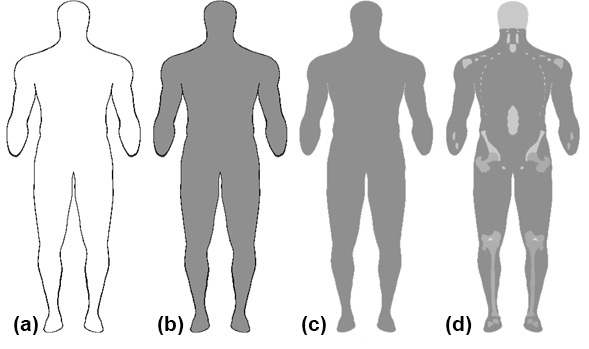
\includegraphics[width=0.7\textwidth]{IMG/Volume2.png}
    \caption{
    Cortes coronales de la imagen volumétrica en las distintas etapas del proceso de \emph{voxelización}\todo{me gusta esta separación. Usala en el texto. Fase 1 voxelización, fase tetraedrización}.}
\label{fig:voxelizacion}
\end{figure}


Una vez que la imagen 3D ha sido construida, se utiliza para crear una malla de tetraedros \el{asociada}. \del{Este paso intermedio es el que permite animar modelos volumétricos de tal forma que si en vez de llegar como entrada una malla superficial, una representación volumétrica podría servir con el mismo fin.}
Para crear la malla de tetraedros se utiliza el algoritmo \ac{RDT} \cite{jamin:hal-00796052}. Este algoritmo permite generar mallas de tetraedros multidominio \del{(segmentadas)} a partir de mallas superficiales o imágenes 3D. \new{A la hora de }\del{Con el objetivo} de configurar el algoritmo, se debe alcanzar un compromiso entre precisión y eficiencia (ver anexo \ref{anexo:criterios}). Se ha configurado para incrementar los tetraedros alrededor de la piel y la superficie de los huesos. Para la realización de esta tesis, se ha conseguido mantener el número de los tetraedros por debajo de $3.5\times 10^6$ y el número de vértices por debajo de $8 \times 10^5$. Destacar que la malla de tetraedros \del{es}\new{se} etiquetada usando los tejidos \del{de los huesos}\new{oseos} y la piel (Fig. \ref{fig:tetra}).
%
\begin{figure}[th]
   \centering
    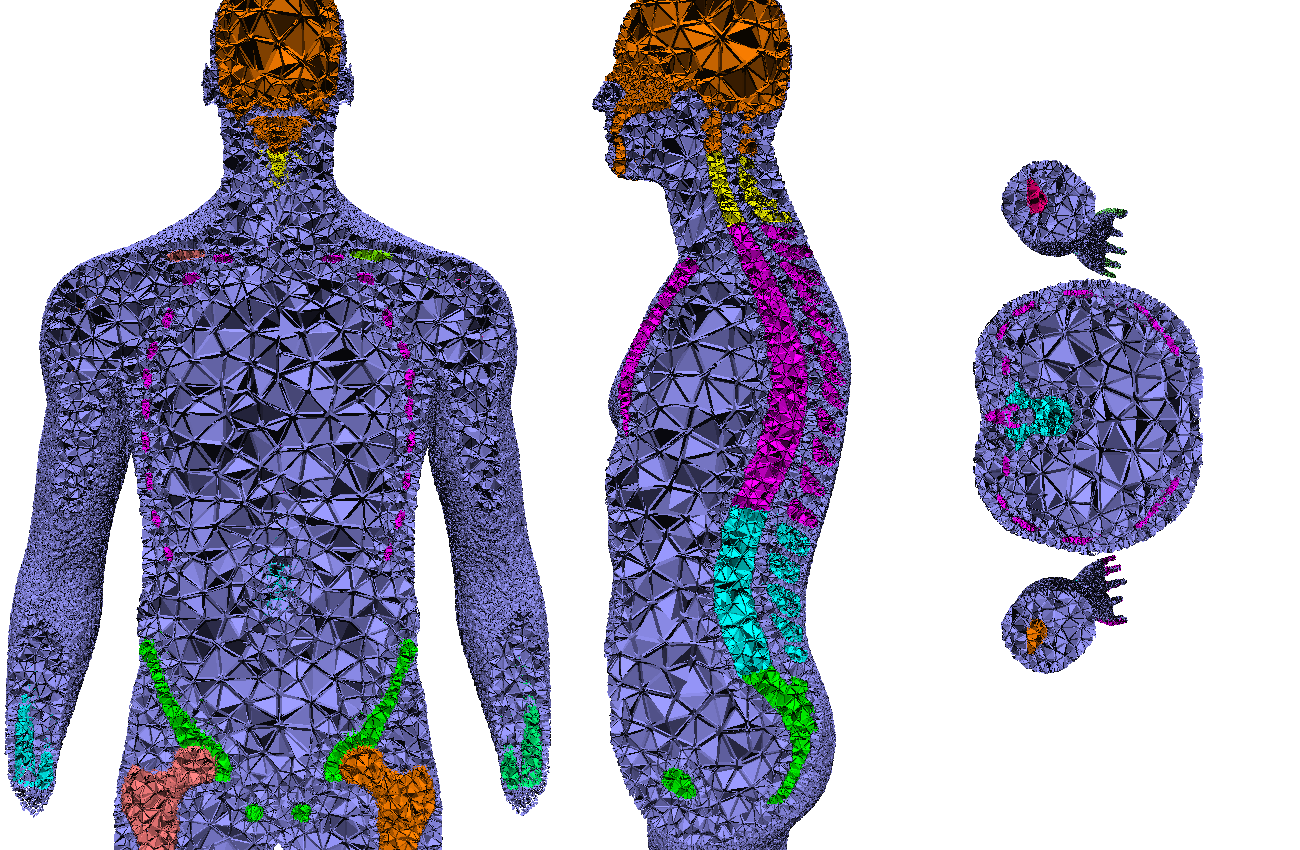
\includegraphics[width=0.5\textwidth]{IMG/boneid.png}
     \caption{Cortes coronales, sagitales y axiales mostrando el resultado de la volumetrización (\new{(restultados de la tetraedrización)}). Los tetraedros etiquetados como huesos se muestran en diferentes colores.}
\label{fig:tetra}
\end{figure} 

%%%%%%%%%%%%%%%%%%%%%%%%%%%%%%%%%%%%%%%%%%%%%%%%%%%%%
\subsection{Pesado}
\label{posing:Pesado}
%%%%%%%%%%%%%%%%%%%%%%%%%%%%%%%%%%%%%%%%%%%%%%%%%%%%%%
%
Como se ha introducido en el estado del arte (ver sección \ref{art:pesado}), la etapa de pesado es dónde se calcula \new{como influye el movimiento de cada hueso sobre los vértices de la malla superficial.}\del{la influencia de cada hueso virtual a los vértices de la malla superficial.} En el caso de este nuevo algoritmo, hay que hacer una serie de cambios para adaptarlo al campo de desplazamientos calculada en la etapa anterior\todo{En el paso anterior no se calculó un campo de desplazamientos. Volumetrizó el espacio interior. El pesado calcula la influencia de los huesos sobre los vértices. Esta influencia se usa para mover los vértices siguiendo el movimiento de los huesos. Una ve que se han movido los vértices se calcula el campo de desplazamientos en el interior de cada tetraedro interpolando mediante coordenadas baricéntricas el desplazamiento de los vértices. En resumen la frase es confusa cambiala}. Así pues, en este caso se va a calcular la influencia de los huesos reales y no de los huesos virtuales a los vértices de la malla de tetraedros y no de los vértices de los distintos tejidos\todo{Separa las ideas. La primera diferencia es que no se usa el esquelto virtual, sino que se propaga la influencia del tejido oseo. Diferencia 2, no se calcula la influencia sobre el resto de tejidos sino que se calcuala la influencia sobre los vertices de la malla volumetrica}. 


Al igual que \new{los algoritmos de pesado clasicos,}\del{el pesado para mallas superficiales,} los pesos calculados para los vértices de los tetraedros tienen que cumplir las mismas condiciones que se citan en \ref{cond1} y \ref{cond2}.
\emph{Baran y Popovi\'{c}} en \cite{Baran:2007} presentan un trabajo que realiza el pesado de forma automática y crea transiciones suaves entre articulaciones. Ellos proponen usar la ecuación de difusión laplaciana suponiendo que la influencia de los huesos se propaga a través del modelo al igual que haría la temperatura. Existen actualmente técnicas para calcular el pesado de forma más efectiva \cite{Jacobson:2011} comentadas en el estado del arte, pero se basan en el mismo principio\todo{que no se basen en el mismo principio no es suficiente para descartarlas}. Tomando en cuenta la idea original de \emph{Baran y Popovi\'{c}}\cite{Baran:2007}, se ha modificado\todo{que se ha modificado} para adaptarla al algoritmo propuesto debido a que su aplicación no es directa\todo{reescribe la frase}. Este algoritmo  sólo puede ser aplicado a mallas superficiales y tienen que contener completamente al esqueleto virtual\todo{1. Rehaz la pasiba. Que es lo que tiene que contener el esqueleto virtual}. Por tanto, se necesita adaptar estas técnicas al algoritmo propuesto teniendo una malla volumétrica como objetivo\todo{la frase no suena bien}. Se propone resolver la ecuación \ref{diffusion} de forma que la solución propuesta hace que la energía laplaciana sea estacionaria. \todo{reescribe la frase. Da la sensación que no entiendes que escribes. 1 Reformulamos el problemas haciendo cero el laplaciano. Esto es equivalente a minizar la energia. }
%and our solutions make the Laplacian energy functional stationary.
Además, esta adaptación asegura una suavidad de orden superior\todo{la frase no suena bien}. Por otra parte, la formulación propuesta lleva a resolver un sistema de ecuaciones lineales, mientras que la técnica presentada en \cite{Jacobson:2011} requiere resolver un problema disperso y cuadrático para imponer las restricciones. \nuevo{revisar Marcos. No suena bien. Pero no te lo puedo reescribir todo.}
% Therefore, our technique ensures high-order smoothness.  Additionally, our formulation drives to a linear equation system, while this technique requires solving a sparse quadratic programming problem in order to impose the constraint set.
Con el objetivo de calcular los pesos $W_j$ de un hueso $j$, se resuelve el caso estacionario definido en la ecuación \ref{diffusion}\todo{Tengo la impresion de que sueltas frases sin preocuparte de que sigan un orden logico. Esto está muy flojo.}. Para resolver esta ecuación para un hueso $j$, se imponen las siguientes condiciones de contorno: se considera que el valor $W_j$ es $1$ dentro de los tetraedros etiquetados como $j$; y el valor es $W_j$ es $0$ dentro de los tetraedros etiquetados como $k$, donde $k$ es cualquier otro hueso que no es $j$.
%
\begin{equation}
\label{diffusion}
\nabla^{2} W_j = 0.
\end{equation}
%

La anterior ecuación es discretizada\todo{pasiva} usando \ac{FEM} y las coordenadas baricéntricas de los tetraedros se utilizan como función de forma (ver \cite{Lewis2004}). La ecuación \ref{system} muestra la discretización final de la ecuación de difusión:
%
\begin{equation}
\label{system}
\mathbf{A} \mathbf{W}_j = \mathbf{b}_j,
\end{equation}
%
donde $\mathbf{A}$ es la matriz de coeficientes del sistema, el vector $\mathbf{b}_j$ depende de las condiciones de contorno del hueso  $j$ y $\mathbf{W}_j$ es un vector que  contiene los pesos  $w_{i,j}$ para cada vértice sin etiquetar $i$. $\mathbf{A}$ es la misma matriz para cada hueso y es simétrica y definida positiva. Esto permite calcular la descomposición de \emph{Cholesky} de esta matriz una única vez y usarla para resolver el sistema lineal de cada hueso.

Es importante mencionar que esta formulación cumple con las restricciones que se imponen en \ref{cond1} y \ref{cond2}. Primero, el máximo y mínimo valor sólo se alcanzan en los huesos y son $0$ y $1$. Segundo, si se considera $\mathbf{b}=\sum^{n}_{j=0}\mathbf{b}_j $ y $\mathbf{W}=\sum^{n}_{j=0}\mathbf{W}_j $, donde  $n$ es el número de huesos, $\mathbf{A} \mathbf{W} = \mathbf{b}$ describe un sistema donde todos los puntos del contorno tendrán un valor de $1$. Además, como el máximo y el mínimo valor es alcanzado solamente en el contorno, todos los elementos de $\mathbf{W}$ tomarán  $1$, probando la condición \ref{cond2}.

\todo{no coloreas los vertices}
 \begin{figure}[h]
   \centering
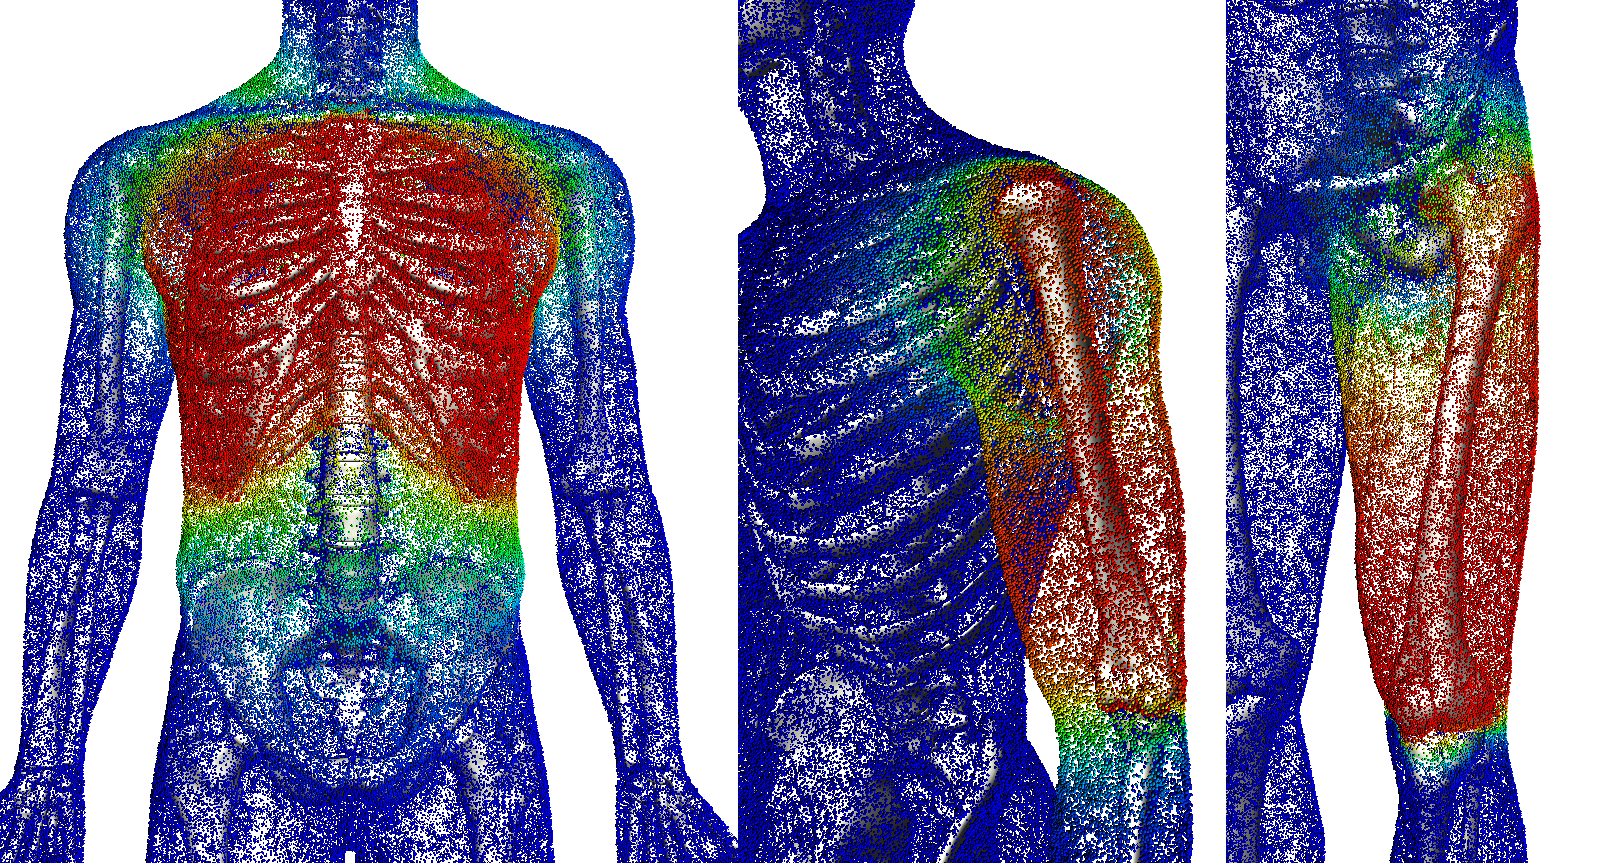
\includegraphics[width=0.49\textwidth]{IMG/weights.png}
     \caption{Vértices de la malla de tetraedros coloreados según la influencia de cada hueso.}
      \label{fig:pesado}
\end{figure}
 
En la figura \ref{fig:pesado} se puede observar la influencia de la caja torácica, el húmero y el fémur en los vértices de la malla de tetraedros. Las zonas rojas muestran valores cercanos a 1 y las zonas azules cercanas a 0. 






%%%%%%%%%%%%%%%%%%%%%%%%%%%%%%%%%%%%%%%%%%%%%%%%%%%
\subsection{Mapeado}
\label{posing:Mapeado}
%%%%%%%%%%%%%%%%%%%%%%%%%%%%%%%%%%%%%%%%%%
%
Para poder transferir los movimientos de las articulaciones virtuales a los tejidos del modelo, hay que vincular éstos con los tetraedros de la malla de volumétrica generada en la etapa de volumetrización. De esta forma se relaciona cada vértice de las mallas superficiales con un tetraedro consiguiendo que el campo de desplazamientos definido por la malla de tetraedros sea trasladado a todos los tejidos que se pretendan animar.\todo{Tus frases no suenan naturales}

Se puede parametrizar la posición del vértice que ocupa dentro de su tetraedro asociado con ayuda de las coordenadas baricéntricas. Estas coordenadas indican la influencia de cada uno de los vértices del tetraedro al vértice que esta mapeado. Por tanto, hay que calcular cada una de las coordenadas baricéntricas para cada vértice de las mallas superficiales.

El enfoque más simple es comprobar cada $n$ vértices con cada $m$ tetraedros. Eso significa que la complejidad de comprobar uno a uno es de $\mathcal{O}(n\ m)$. Para acelerar el cálculo global, se ha utilizado una \ac{tabla hash} \cite{Teschner2003} para subdividir la malla de tetraedros\todo{la técnica es espacial hashing}. En vez de comprobar uno por uno de los tetraedros de la malla, solo se comprobarán aquellos que están cerca utilizando la \ac{tabla hash} para acceder de manera inmediata. De esta manera se ha reducido desde horas que tarda el método de fuerza bruta hasta poder calcular todo el mapeado en menos de un minuto. En el caso de que algún vértice quede fuera de la malla de tetraedros, la misma \ac{tabla hash} facilitará la búsqueda del tetraedro más cercano.
\todo{No esta bien explicado}


%%%%%%%%%%%%%%%%%%%%%%%%%%%%%%%%%%%%%%%%%%%%%%%%%%%%%%
\subsection{Selección de poses}
\label{posing:Poses}
%%%%%%%%%%%%%%%%%%%%%%%%%%%%%%%%%%%%%%%%%%%%%%%%%%%%%%
%
En esta etapa, el usuario es el encargado de seleccionar interactivamente la posición que se quiera trasladar al personaje virtual. El algoritmo desarrollado en esta tesis permite usar cinemática directa, poses pregrabadas y animaciones, incluso usar el dispositivo \emph{Microsoft Kinect}~\cite{shotton2013} para capturar la pose del usuario y transferirla al paciente virtual. Aun así, técnicas como \emph{retargeting} \cite{7581666} o cinemática inversa, puede ser incluidas en el algoritmo.\todo{el pueden ser incluidas suena mal.}

Para transferir la animación esqueletal a una malla superficial se utiliza el modelo matemático llamado \emph{skinning} como se ha podido leer anteriormente en el estado del arte (sec.\ref{art:skinning})\todo{el skinning no es un modelo matematico, son los algoritmos que transfieren el movimiento de los usos... Tal y como esta redacto parece que en el estado del arte has anticipado que TU ALGORITMO USARA EL SKINNING}. En el caso del algoritmo propuesto, se puede tratar los vértices de los tetraedros como vértices de una malla superficial\new{????}. De la misma manera que la animación clásica las animaciones esqueletales son transferidas a la malla volumétrica usando una técnica de \emph{skinning}. Los tetraedros deformados definen un campo de deformación que se utiliza para animar todos los tejidos del paciente virtual.
\todo{A partir de ahora solo voy a dar pinceladas. Llevo la mañana del viernes, la del sabado y la del domingo y no avanzo. No puedo comentar cada frase. Es TU RESPONSABILIDAD cuidar la redacción. }


Se ha elegido implementar la técnica de \emph{skinning} descrita en \cite{le2016real}. Se ha decidido usar la técnica \ac{COR} ya que resuelve algunos de los problemas de \ac{DQS} y \ac{LBS} como se ha descrito anteriormente y es totalmente compatible con el cauce clásico de la animación esqueletal. \emph{Le y Hodghins} calcula unos centros de rotación óptimos para todos los vértices de la malla de tetraedros\todo{paredce que son ellos trabajan con mallas de tetrahedros}. Una vez esta información es calculada, esta técnica no afecta al rendimiento del sistema en comparación con las otras dos técnicas. Estas tres técnicas son intercambiables entre si debido a que están perfectamente diseñadas para usarse con las arquitecturas gráficas modernas. Este algoritmo está basado en que los vértices con un pesado similar deben seguir las mismas transformaciones. En su trabajo, \emph {Le y Hodgins} ~\cite{le2016real} proponen la función de similaridad que se muestra a continuación:
\todo{pasivas, intercambiables????}

%\begin{eqnarray}\nonumber
\begin{equation}
 s(\textbf{w}_p,\textbf{w}_s) = 
\sum_{\forall i \neq j} w_{p,i}w_{p,j}w_{s,i}w_{s,j}\exp-\frac{(w_{p,i}w_{s,j}-w_{s,i}w_{p,j})^2}{\sigma^2}
\end{equation}
%\end{eqnarray}
\normalsize
%
donde $\textbf{w}_p$ y $\textbf{w}_s$ son vectores de los pesos de los vértices $p$ y $s$, y $\sigma$ es el parámetro de configuración. Esta función es usada para calcular el nuevo centro de rotación. Se ha adaptado la ecuación propuesta en \cite{le2016real} para tratar con la malla de tetraedros en vez de mallas de triángulos de la siguiente manera: 
%
\begin{equation}
%\begin{eqnarray}\nonumber
\textbf{cor}_p = 
\frac
  {
  \sum_{\forall t \in T}
    s(\textbf{w}_p,
      \frac{\textbf{w}_{t1}+\textbf{w}_{t2}+\textbf{w}_{t3}+\textbf{w}_{t4}}{4})
    %\frac{\textbf{v}_{t1}+\textbf{v}_{t2}+\textbf{v}_{t3}+\textbf{v}_{t4}}{4}
    V_t\mathbf{c}_t
  }
  {
  \sum_{\forall t \in T}
    s(\textbf{w}_p,
      \frac{\textbf{w}_{t1}+\textbf{w}_{t2}+\textbf{w}_{t3}+\textbf{w}_{t4}}{4})
    V_t
  } 
%\end{eqnarray}
\normalsize
\end{equation}
%
donde $\textbf{cor}_p$ es el nuevo centro de rotación del vértice $p$, $t$ es el tetraedro de la malla de tetraedros $T$, $V_t$ es el volumen del tetraedro $t$, $\textbf{c}_t$ es el centroide del tetraedro $t$ y $\textbf{w}_{t1}$, $\textbf{w}_{t2}$, $\textbf{w}_{t3}$ y $\textbf{w}_{t4}$ son los pesos de los vértices del tetraedro $t$. Una vez calculado este centro, puede ser usado en la etapa interactiva utilizando el \emph{shader} descrito en \cite{le2016real}.\todo{pasiva}

\todo{pasiva}
El campo de desplazamiento de un punto dentro de un tetraedro puede ser calculado interpolando el desplazamiento de cada uno de sus vértices. Se interpola este campo usando las coordenadas baricéntricas de cada tetraedro, ya calculadas en el paso de pesado (sec. \ref{posing:Pesado}). Matemáticamente, el campo de desplazamientos calculado es continuo pero no diferenciable dentro de la malla volumétrica y permite calcular una matriz de transformación constante por cada tetraedro (consultar \cite{Muller2004}). \todo{pasiva} Esta matriz de transformación, perteneciente al tetraedro, es aplicada a cada uno de los vértices de la malla superficial asociados al tetraedro. Estos cálculos se realizan en la tarjeta gráfica para mejorar el rendimiento del algoritmo.\todo{pasiva}.

\todo{No se si este apartado se entiende lo basta bien. Es muy criptioco. No se si tu contribución esta clara}


% %%%%%%%%%%%%%%%%%%%%%%%%%%%%%%%%%%%%%%%%%%%%%%%%%%%%%%
 \subsection{Optimización}
\label{posing:optimizacion}
% %%%%%%%%%%%%%%%%%%%%%%%%%%%%%%%%%%%%%%%%%%%%%%%%%%%%%%
% %
% \marginpar{A tenor de los resultados hay que ver si esta etapa tiene sentido!}
% %

Los resultados de la etapa previa son visualmente realistas\todo{¿Como lo sabes?}. \ac{COR} reduce el volumen ganado por \ac{DQS} o el volumen perdido por \ac{LBS}\todo{tienes resultados que lo respalden}. Aun así, hay algunos escenarios dónde se produce un cambio apreciable de volumen. El algoritmo propuesto permite al usuario refinar la solución usando un algoritmo basado en físicas. Al no disponer de todos los tejidos o de las propiedades mecánicas, el objetivo de esta etapa es mejorar el aspecto visual del resultado asegurando la conservación del volumen. \todo{Esta asunción suena raro}Esta asunción es debido que se puede decir que todos los tejidos están compuestos de agua y se asume que es un fluido incompresible y por tanto, las deformaciones tienen que permitir la conservación de volumen para cada tetraedro.\todo{Parce que los tejidos son solo agua.}


\todo{ponemos fórmulas que tenías en los comentarios?}
\todo{Si eres capaz de explicarlo...}


Para resolver la conservación del volumen de cada tetraedro se plantea el siguiente modelo mecánico que se caracteriza por: plantear las ecuaciones del equilibrio estático, emplear el tensor de deformaciones de \emph{Cauchy} y emplear un modelo de elasticidad isotrópico, homogéneo y lineal. Para utilizar el tensor de deformaciones de \emph{Cauchy} sin problemas derivados\todo{derivado de que?}, se utilizará la formulación co-rotacional del \ac{FEM} para resolver el sistema. En la etapa de \emph{volumetrización} (sec. \ref{posing:volumetrizacion}) será utilizada como discretización espacial y las posiciones de los huesos se pueden utilizar como \new{las} condiciones de contorno necesarias para resolver el problema estático. Puede encontrase información adicional en \cite{Muller2004}. \todo {pasivas}

\todo{No es el Fem lo que se configura}
El método \ac{FEM} es habitualmente configurado a través de dos parámetros: el \emph{ratio de Poisson} y el \emph {módulo de Young}. El \emph{ratio de Poisson} controla la conservación de volumen y para garantizar dicha conservación se debe de tomar un valor de 0.5 (el valor real utilizado es ligeramente inferior a 0.5 para asegurar la estabilidad numérica). El \emph {módulo de Young} es el parámetro que caracteriza el comportamiento de un material elástico, según la dirección en la que se aplica una fuerza. En este caso, este parámetro no será especialmente importante debido a que \todo{sigue??????? Pasiva}. En este caso será útil elegir un valor con el objetivo de mejorar la estabilidad numérica del sistema. Para ello habría\todo{habría que o lo has hecho} que analizar la matriz de coeficientes del sistema para varios valores del módulo y seleccionar aquel valor que dé como resultado la matriz de coeficientes con menor número condicionante.

Respecto a la formulación co-rotacional se basa en calcular en una configuración no rotada las fuerzas internas (derivadas de la deformación) y que se usarán después rotándolas a la configuración final \cite{Muller2004}. Primero, es necesario calcular la rotación \del{final} de los elementos de la malla de tetraedros. Como esta rotación se desconoce, el problema estático se puede resolver de forma iterativa. Se utiliza la deformación inicial en los tetraedros como situación inicial para reducir significativamente el número de iteraciones requeridas para llegar a la solución final.  %(ver Fig. \ref{x}). 

Para conocer los desplazamientos de los vértices de la malla de tetraedros se ha formulado un sistema de ecuaciones lineales. Según las propiedades anteriormente citadas, la matriz de coeficientes del sistema lineal es dispersa, simétrica y definida positiva. Este tipo de sistemas de ecuaciones se pueden resolver utilizando el método del gradiente conjugado \cite{Press2007}. La convergencia de estos métodos se acelera con el uso de pre-condicionadores (ver \cite{hauth2003}) y utilizando como solución inicial una cercana a la solución final. Para acelerar esta etapa, se utiliza  como solución inicial la posición del modelo ya calculado en la etapa de selección de poses (sec. \ref{posingPoses}), además de emplear un precondicionador de Jacobi.

Finalmente, los desplazamientos realizados por los tetraedros se utilizarán, en un segundo paso, para calcular la transformación que se aplicará a todos los tejidos asociados a cada tetraedro (ver sec. \ref{posing:Poses}). 



%%%%%%%%%%%%%%%%%%%%%%%%%%%%%%%%%%%%%%%%%%%%%%%%%%%%%%%%%
\section{Detalles de implementación}
\label{posing:preprocess}
%%%%%%%%%%%%%%%%%%%%%%%%%%%%%%%%%%%%%%%%%%%%%%%%%%%%%%%%%

\todo{seccion dos veces en la misma frase. }
Como se puede leer en la sección de requisitos (sec. \ref{posing:req}), la selección de poses debe ser supervisada por un usuario y por tanto la animación del modelo debe ser interactiva. La etapa de \emph{selección de poses} debe cumplir con ello lo que lleva a realizar las demás etapas en un proceso previo al poder utilizar el modelo virtual.\todo{la frase anterior es horrible. Esta parte final de la memoria esta poco cuidada} Las etapas de \emph{rigging}\todo{esqueletizado}, \emph{volumetrización}, \emph{pesado}, \emph{mapeado} y el cálculo de los centros de rotación son las etapas más costosas computacionalmente, de tal manera que se han relegado \del{al}\new{a un} proceso previo para evitar no poder cumplir con el requisito de interactividad. Estas etapas solo se realizan una vez por modelo virtual y son guardadas en ficheros adjuntos al modelo.\todo{las etapas no se guardan sino sus resultados!} 
Por otra parte, la etapa de \emph{optimización} no es posible que se ejecute en un tiempo razonable para conseguir interacción en tiempo real dependiendo del tamaño de la malla volumétrica resultante. Se deja a elección del usuario cuando se procede a ejecutar esta etapa.


